                                        % abtex2-modelo-artigo.tex, v-1.9.2 laurocesar
% Copyright 2012-2014 by abnTeX2 group at http://abntex2.googlecode.com/ 
%

% ------------------------------------------------------------------------
% ------------------------------------------------------------------------
% abnTeX2: Modelo de Artigo Acadêmico em conformidade com
% ABNT NBR 6022:2003: Informação e documentação - Artigo em publicação 
% periódica científica impressa - Apresentação
% ------------------------------------------------------------------------
% ------------------------------------------------------------------------

\documentclass[
	% -- opções da classe memoir --
	article,			% indica que é um artigo acadêmico
	11pt,				% tamanho da fonte
	oneside,			% para impressão apenas no verso. Oposto a twoside
	a4paper,			% tamanho do papel. 
	% -- opções da classe abntex2 --
	%chapter=TITLE,		% títulos de capítulos convertidos em letras maiúsculas
	%section=TITLE,		% títulos de seções convertidos em letras maiúsculas
	%subsection=TITLE,	% títulos de subseções convertidos em letras maiúsculas
	%subsubsection=TITLE % títulos de subsubseções convertidos em letras maiúsculas
	% -- opções do pacote babel --
	english,			% idioma adicional para hifenização
	brazil,				% o último idioma é o principal do documento
	sumario=tradicional
	]{abntex2}


% ---
% PACOTES
% ---

% ---
% Pacotes fundamentais 
% ---
\usepackage{lmodern}			% Usa a fonte Latin Modern
\usepackage[T1]{fontenc}		% Selecao de codigos de fonte.
\usepackage[utf8]{inputenc}		% Codificacao do documento (conversão automática dos acentos)
\usepackage{indentfirst}		% Indenta o primeiro parágrafo de cada seção.
\usepackage{nomencl} 			% Lista de simbolos
\usepackage{color}				% Controle das cores
\usepackage{graphicx}			% Inclusão de gráficos
\usepackage{microtype} 			% para melhorias de justificação
\usepackage{eurosym}            % para acrescentar o símbolo do EURO
\usepackage{float}
% ---
		
% ---
% Pacotes adicionais, usados apenas no âmbito do Modelo Canônico do abnteX2
% ---
\usepackage{lipsum}				% para geração de dummy text
% ---
		
% ---
% Pacotes de citações
% ---
\usepackage[brazilian,hyperpageref]{backref}	 % Paginas com as citações na bibl
\usepackage[alf]{abntex2cite}	% Citações padrão ABNT
% ---

% ---
% Configurações do pacote backref
% Usado sem a opção hyperpageref de backref
\renewcommand{\backrefpagesname}{Citado na(s) página(s):~}
% Texto padrão antes do número das páginas
\renewcommand{\backref}{}
% Define os textos da citação
\renewcommand*{\backrefalt}[4]{
	\ifcase #1 %
		Nenhuma citação no texto.%
	\or
		Citado na página #2.%
	\else
		Citado #1 vezes nas páginas #2.%
	\fi}%
% ---

% ---
% Informações de dados para CAPA e FOLHA DE ROSTO
% ---
\titulo{Desenvolvendo um Sistema Especialista voltado para Teste Vocacional}
\author{Cassiane Nodari
\thanks{Acadêmica de Ciência da Computação - URI Erechim \{51140@aluno.uricer.edu.br}}
\local{Brasil}
%\data{}
% ---

% ---
% Configurações de aparência do PDF final

% alterando o aspecto da cor azul
\definecolor{blue}{RGB}{41,5,195}

% informações do PDF
\makeatletter
\hypersetup{
     	%pagebackref=true,
		pdftitle={\@title}, 
		pdfauthor={\@author},
    	pdfsubject={Modelo de artigo científico com abnTeX2},
	    pdfcreator={LaTeX with abnTeX2},
		pdfkeywords={abnt}{latex}{abntex}{abntex2}{atigo científico}, 
		colorlinks=black,       		% false: boxed links; true: colored links
    	linkcolor=black,          	% color of internal links
    	citecolor=black,        		% color of links to bibliography
    	filecolor=magenta,      		% color of file links
		urlcolor=blue,
		bookmarksdepth=4
}
\makeatother
% --- 

% ---
% compila o indice
% ---
\makeindex
% ---

% ---
% Altera as margens padrões
% ---
\setlrmarginsandblock{3cm}{3cm}{*}
\setulmarginsandblock{3cm}{3cm}{*}
\checkandfixthelayout
% ---

% --- 
% Espaçamentos entre linhas e parágrafos 
% --- 

% O tamanho do parágrafo é dado por:
\setlength{\parindent}{1.3cm}

% Controle do espaçamento entre um parágrafo e outro:
\setlength{\parskip}{0.2cm}  % tente também \onelineskip

% Espaçamento simples
\SingleSpacing

% ----
% Início do documento
% ----
\begin{document}

% Retira espaço extra obsoleto entre as frases.
\frenchspacing 

% ----------------------------------------------------------
% ELEMENTOS PRÉ-TEXTUAIS
% ----------------------------------------------------------

%---
%
% Se desejar escrever o artigo em duas colunas, descomente a linha abaixo
% e a linha com o texto ``FIM DE ARTIGO EM DUAS COLUNAS''.
% \twocolumn[    		% INICIO DE ARTIGO EM DUAS COLUNAS
%
%---
% página de titulo
\maketitle



 				% FIM DE ARTIGO EM DUAS COLUNAS
% ---

% ----------------------------------------------------------
% ELEMENTOS TEXTUAIS
% ----------------------------------------------------------
\textual

% Doc no drive https://docs.google.com/document/d/12J5yA2UA_die099Nc6DNkkvGKVc7e_fbe8Y-lV4SN54/edit

% ----------------------------------------------------------
% Introdução
% ----------------------------------------------------------
\section*{Introdução}
\addcontentsline{toc}{section}{Introdução}
A inteligência artificial é uma inovação que vem sendo estudada cada dia mais e trata-se de como as máquinas possuem capacidade de aprender, raciocinar e perceber como seres humanos.

Com base nisso foi elaborado este trabalho que tem por objetivo abordar um dos temas da Inteligência Artifical chamado de Sistemas Especialistas, bem como explicar como é o funcionamento, em qual área de conhecimento ele é utilizado, além de exemplificar um sistema especialista com uma implementação prática. 

Um teste vocacional trata-se da escolha de um determinado curso de gradução à ser feito, através dos níveis de interesse que o usuário possui. Muitos estudantes saem do ensino médio sem ter um curso pretendido para cursar, por isso o teste vocacional está apto a ajudar na escolha certa. Motivado pelo problema comum de pessoas que precisam escolher um curso para realizar os estudos e muitas vezes ficam com dúvida em quanto será gasto e se escolherá o curso certo que atenda seus níveis de interesse é que foi realizado esta pesquisa e implementação prática.

Na seção primária \ref{sistemaespecialista}, será tratrado de explicar o que é um sistema especialista e como ele funciona.

A seção secundária \ref{expertsinta} descreve o que é o expert sinta e suas principais telas

Na seção primária \ref{metodologia} está o desenvolvimento do sistema especialista juntamente com a metodologia utilizada.

Na seção primária \ref{discussão} é tratado as discussões e análises dos resultados encontrados durante os estudos da ferramento e do sistema especialista.

Na seção primária \ref{conclusao} trata-se do que foi concluído com o desenvolvimento do trabalho.

% ----------------------------------------------------------
% Seção de explicações
% ----------------------------------------------------------
\section{Referencial Teórico}
\subsection{O Sistema Especialista}
\label{sistemaespecialista}

A partir da construção de uma base de conhecimento,  motor de inferência e de um especialista, o sistema é capaz de realizar soluções esperadas por seres humanos. Estimula-se uma série de regras nas quais determinam alguns fatores importantes para que o sistema possa tomar uma decisão sobre o determinado assunto, e então é trazido o possível resultado encontrado pelo sistema com base nas respostas do usuário.

Da mesma forma que ocorre com as pessoas, para que uma pessoa seja especialista em uma área específica, ela precisa estudar, treinar e se aprofundar  neste assunto para se tornar especialista naquilo.
O sistema especialista geralmente é alimentado por uma pessoa especialista em determinada área e utiliza os requisitos citados acima para se tornar um especialista na tomada de decisão e descobrir a resposta correta que o usuário precisa, sem ter de pedir uma resposta exata daquilo que ele deve encontrar. \cite{Jones}

É uma área da Inteligência Artificial muito usada na área da saúde, principalmente por médicos, para facilitar na descoberta por doenças e ter auxílio para dar a pescrição médica ao paciente. Conforme cita \citeonline{Renato}, "os sistemas especialistas estão sendo utilizados de forma rotineira em muitos setores da atividade humana".
Empresas que trabalham com transações de cartão precisam ter uma decisão rápida de aprovação ou não, e por este motivo também é utilizado este conceito.

\begin{figure}[H]
    \centering
    \caption{Processo de um sistema especialista}
    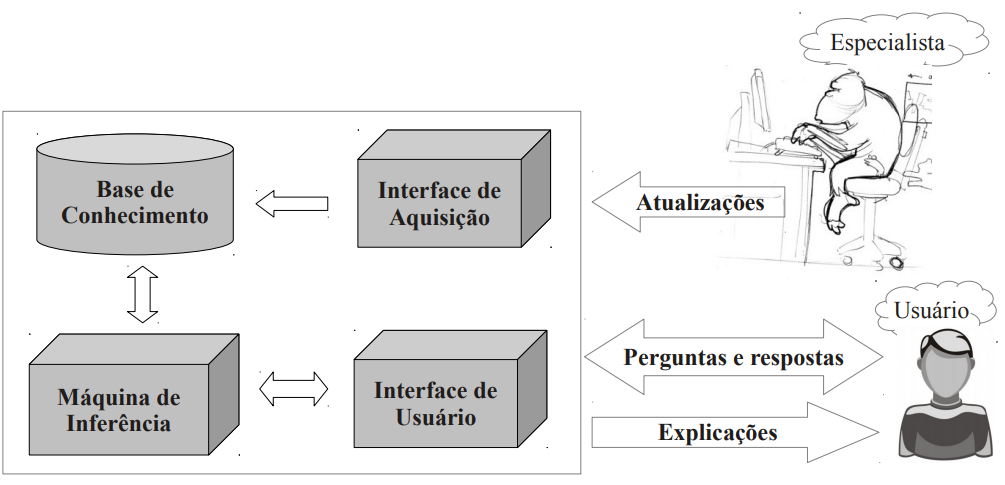
\includegraphics[width=0.8\textwidth]{figura1.PNG}
    \label{processosistema}
    \fonte{\cite{jacsonsilva}}
\end{figure}

A base de conhecimento é o local onde ficam salvas as regras e os fatos. Onde pode ser estruturado e codificado de qualquer maneira para que atinja os resultados desejados.

O motor de inferência ou mecanismo de inferência como também pode ser chamado, pode ser melhor explicado por
\cite{antoniopereira} "É o processo ou interpretação do conhecimento sendo considerado, o coração do mesmo. A principal função é combinar o conhecimento abstrato contido na base regras com o conhecimento concreto armazenado na base de fatos, inferindo conclusão e gerando novos fatos".

Interface do usuário, também possui um papel importante que é realizar a comunição com o usuário através de perguntas e respostas.

O mecanismo de base do interpretador utiliza o encadeamento para frente (\textit{forward}) e encadeamento para trás (\textit{backward}). \citeonline{jacsonsilva} descreve a diferença entre os encadeamentos.

\begin{itemize}
    \item Encadeamento para frente, controle progressivo ou \textit{forward-chaining}: as regras são no sentido condições-conclusões. Dadas as regras, tenta-se usá-las como evidências para construir novos conhecimentos.
    \item Encadeamento para trás: controle regressivo ou \textit{backward-chaining} raciocínio guiado por um
objetivo. Usa-se das regras da base de conhecimento para responder as perguntas. Regras no sentido conclusões-condições.
\end{itemize}

\begin{figure}[H]
    \centering
    \caption{Encadeamento forward e backward}
    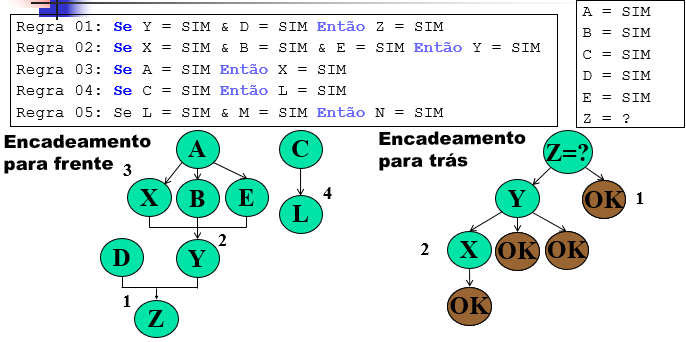
\includegraphics[width=0.8\textwidth]{encadeamento.PNG}
    \label{encadeamento}
    \fonte{\cite{anne}}
\end{figure}


\subsection{Expert Sinta}
\label{expertsinta}

O expert sinta foi desenvolvido pelo  Laboratório de Inteligência Artificial da Universidade Federal do Ceará e é muito conhecido quando se trata de sistemas especialistas. É um software \textit{open source} que foi desenvolvido à algum tempo, mas que por ser muito fácil de utilizar se torna uma ferramenta de grande valor. \cite{Jones}

O software possui interfaces para a manipulação de regras, especificação dos objetivos e criação das variáveis. Possui uma tela para que seja possível observar por quais regras o sistema especialista está passando e deixando gravado as respostas que o usuário informa.

Sistema especialista é baseado em regras que são basicamente conjunto de palavras e fatos com condições e conclusões. É atribuído variáveis para a base de conhecimento e também é estipulado um ou mais objetivos, sendo assim, o processo é iniciado fazendo a pesquisa sobre as regras que possuem o objetivo informado e vai fazendo um encadeamento diante das outras regras até que o seu objetivo realmente seja atingido e então retorna a resposta ao usuário.

Abaixo estão algumas imagens que representam as telas do software, juntamente com exemplos desenvolvidos no trabalho.

% \begin{figure}[H]
%     \centering
%     \caption{Criação de Regras}
%     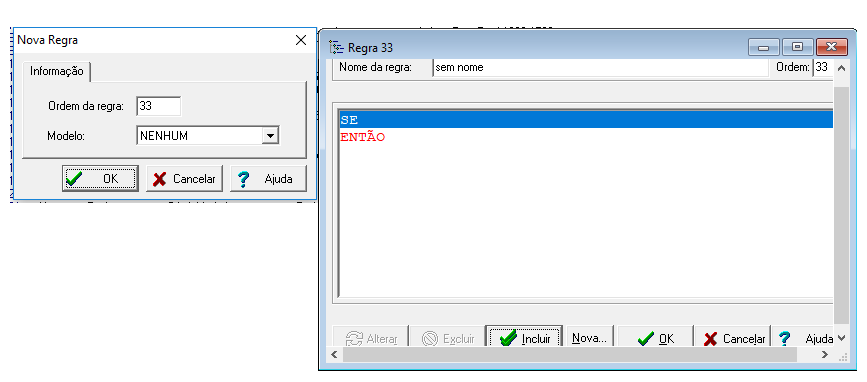
\includegraphics[width=0.8\textwidth]{regra1.PNG}
%     \label{regras1}
%     \fonte{Autor}
% \end{figure}

% \begin{figure}[H]
%     \centering
%     \caption{Consulta de regras criadas}
%     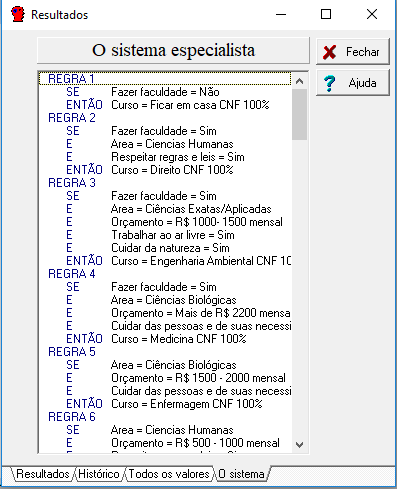
\includegraphics[width=0.8\textwidth]{regras2.PNG}
%     \label{regras2}
%     \fonte{Autor}
% \end{figure}

\begin{figure}[H]
    \centering
    \caption{Regra existente no sistema desenvolvido}
    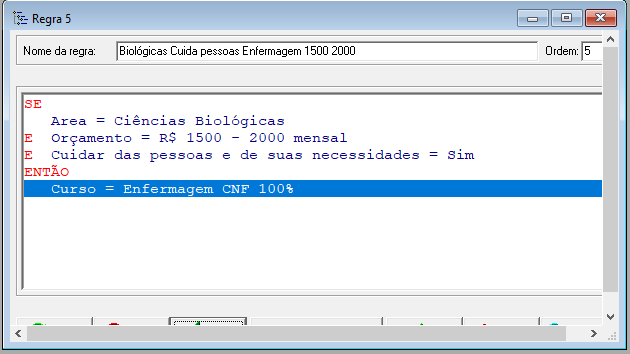
\includegraphics[width=0.8\textwidth]{regras.PNG}
    \label{regras}
    \fonte{Autor}
\end{figure}
A figura \ref{regras} mostra uma das regras que foi criada. O padrão normalmente é este, dá-se três condições e a conclusão é o que está dentro do ENTÃO. Neste caso, se o usuário escolher uma área como sendo Ciências Biológicas, selecionando um valor médio de gasto entre 1500 e 2000 reais mensais, e o perfil dele é de gostar de cuidar das pessoas e de suas necessidades, então o sistema entenderá que deve recomendar o curso de Enfermagem.
 
 
 \begin{figure}[H]
    \centering
    \caption{Criação de Variáveis}
    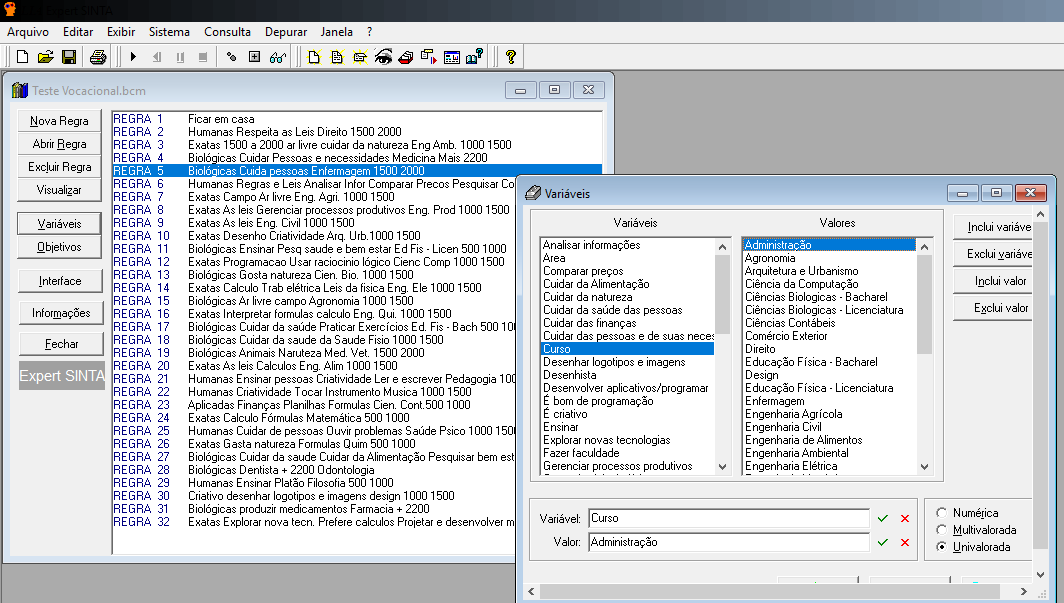
\includegraphics[width=0.8\textwidth]{variaveis.PNG}
    \label{variaveis}
    \fonte{Autor}
\end{figure}
 As variáveis, podem ser criadas para que contenham mais de um único valor, ou seja, marcando a opção multivalorada é possível adicionar mais de um valor à ela.
 
 
  \begin{figure}[H]
    \centering
    \caption{Especificação dos Objetivos}
    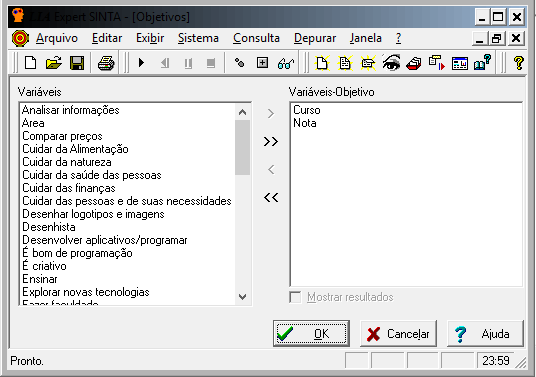
\includegraphics[width=0.8\textwidth]{objetivos.PNG}
    \label{objetivos}
    \fonte{Autor}
\end{figure}

% \begin{figure}[H]
%     \centering
%     \caption{Repostas do usuário}
%     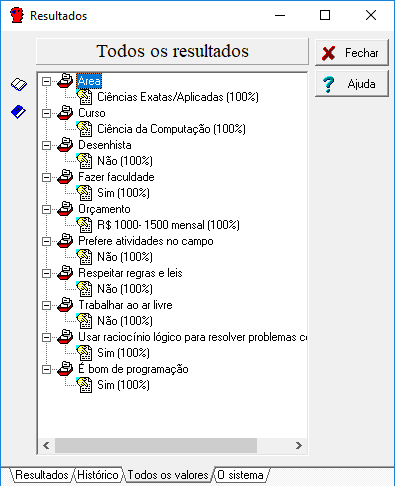
\includegraphics[width=0.5\textwidth]{regras3.PNG}
%     \label{regras3}
% \fonte{Autor}
% \end{figure}

O sistema não irá perguntar diretamente para o usuário sobre a resposta que ele quer, ele irá fazer uma série de outras perguntas, que indiretamente será capaz de descobrir o resultado final, sem que o usuário tenha dito exatamente a sua resposta desejada.


\section{Metodologia}
\label{metodologia}

Utilizou-se a ferramenta Expert Sinta que se encontra no {site}\footnotemark \footnotetext{http://www.lia.ufc.br/~bezerra/exsinta/} para a  realização do trabalho. Levando em conta a facilidade de ser utilizada. Tem por objetivo criar variáveis,  regras com conectivos lógicos e tabelas verdades, assim completando um sistema baseado em conhecimento e fazendo o uso da lógica computacional.




\section{Discussão e Análises dos Resultados}
\label{discussão}
Algumas análises que foram feitas estão baseadas na seguinte regra: para uma pessoa que possui interesse em realizar um curso da área de ciências exatas e gosta de programar, gosta de resolver problemas utilizando raciocínio lógico e pretende gastar um valor médio de 1000,00 a 1500,00, o sistema especialista faz a análise das regras e toma a melhor decisão que é mostrar para o usuário que ele deve realizar o curso de Ciência da Computação. 






% ---
% Conclusão
% ---
\section{Conclusão}
\label{conclusao}


O desenvolvimento deste trabalho permitiu explorar o software Expert Sinta, bem como entender todo o processo realizado pelo sistema especialista para que o valor esperado seja retornado à tela como a melhor solução. A implementação do sistema foi feito através de pesquisas, sobre o funcionamento deste tipo de software e também sobre os fatores mais importantes dentro de cada disciplina de gradução para entender quais seriam as características de cada curso.


% ----------------------------------------------------------
% ELEMENTOS PÓS-TEXTUAIS
% ----------------------------------------------------------
\postextual

% ---
% Título e resumo em língua estrangeira
% ---

% \twocolumn[    		% INICIO DE ARTIGO EM DUAS COLUNAS

% titulo em inglês
% \titulo{Canonical academic article model with \abnTeX}
% \emptythanks
% \maketitle

% % resumo em português
% \renewcommand{\resumoname}{Abstract}
% \begin{resumoumacoluna}
%  \begin{otherlanguage*}{english}
%   According to ABNT NBR 6022:2003, an abstract in foreign language is a back
%   matter mandatory element.

%   \vspace{\onelineskip}
 
%   \noindent
%   \textbf{Key-words}: latex. abntex.
%  \end{otherlanguage*}  
% \end{resumoumacoluna}

% ]  				% FIM DE ARTIGO EM DUAS COLUNAS
% ---

% ----------------------------------------------------------
% Referências bibliográficas
% ----------------------------------------------------------
\bibliography{abntex2-modelo-references}

% ----------------------------------------------------------
% Glossário
% ----------------------------------------------------------
%
% Há diversas soluções prontas para glossário em LaTeX. 
% Consulte o manual do abnTeX2 para obter sugestões.
%
%\glossary

% ----------------------------------------------------------
% Apêndices
% ----------------------------------------------------------

% ---
% Inicia os apêndices
% ---
\begin{apendicesenv}


\end{apendicesenv}
% ---

% ----------------------------------------------------------
% Anexos
% ----------------------------------------------------------
\cftinserthook{toc}{AAA}
% ---
% Inicia os anexos
% ---
%\anexos
\begin{anexosenv}

\end{anexosenv}

\end{document}
